%\begin{equation}
%f_i^{(j,~k)} = \dfrac{\mathbb{E}_i^{(j,~k)}}{\mathbb{E}_i^{(k)}}
%\end{equation}
%de lo cual se deriva que:
%\begin{equation}
%f^{(j,~k)} = \sum_i f_i^{(j,~k)}, ~~~~ f_i^{(k)} = \sum_j f_i^{(j,~k)} ~~~~ y ~~~~~ f^{(k)} = \sum_{ij} f_i^{(j,~k)}
%\end{equation}

Una vez entendida la señal de la teoría \MSSM\textbf{D}, correspondiente a la descomposición según lo muestra el diagrama de la Fig. \ref{fig:sketch_darksector}b, se intenta comprender como los detectores del \CMS ~ en las configuraciones Run-2 y Alta Luminosidad reconstruyen experimentalmente este decaimiento. Para esto la generación de muestras se divide por la simulación de la configuración del detector (ver Tabla \ref{table_genera_v5_value}).

\subsection{Variación del contenido muónico}

Se hace necesario comenzar con la identificación de las variaciones de las distribuciones de frecuencia del número total de muones por evento, según la notación de la ec. \ref{fe} está está denotada por:
\begin{eqnarray}
f^{(\mu, k)}_\textsf{e} (\vec{\alpha}; x) = \sum_{i=1}^{N_e} \delta_{x}(n_i^{(\mu,k)})/N_e
\end{eqnarray}
donde $\vec{\alpha}$ es el vector de parámetros que especifica las condiciones de generación de la señal \MSSM\textbf{D} y $k$ es la configuración del detector requerida.

\begin{figure}[!ht]
\centering
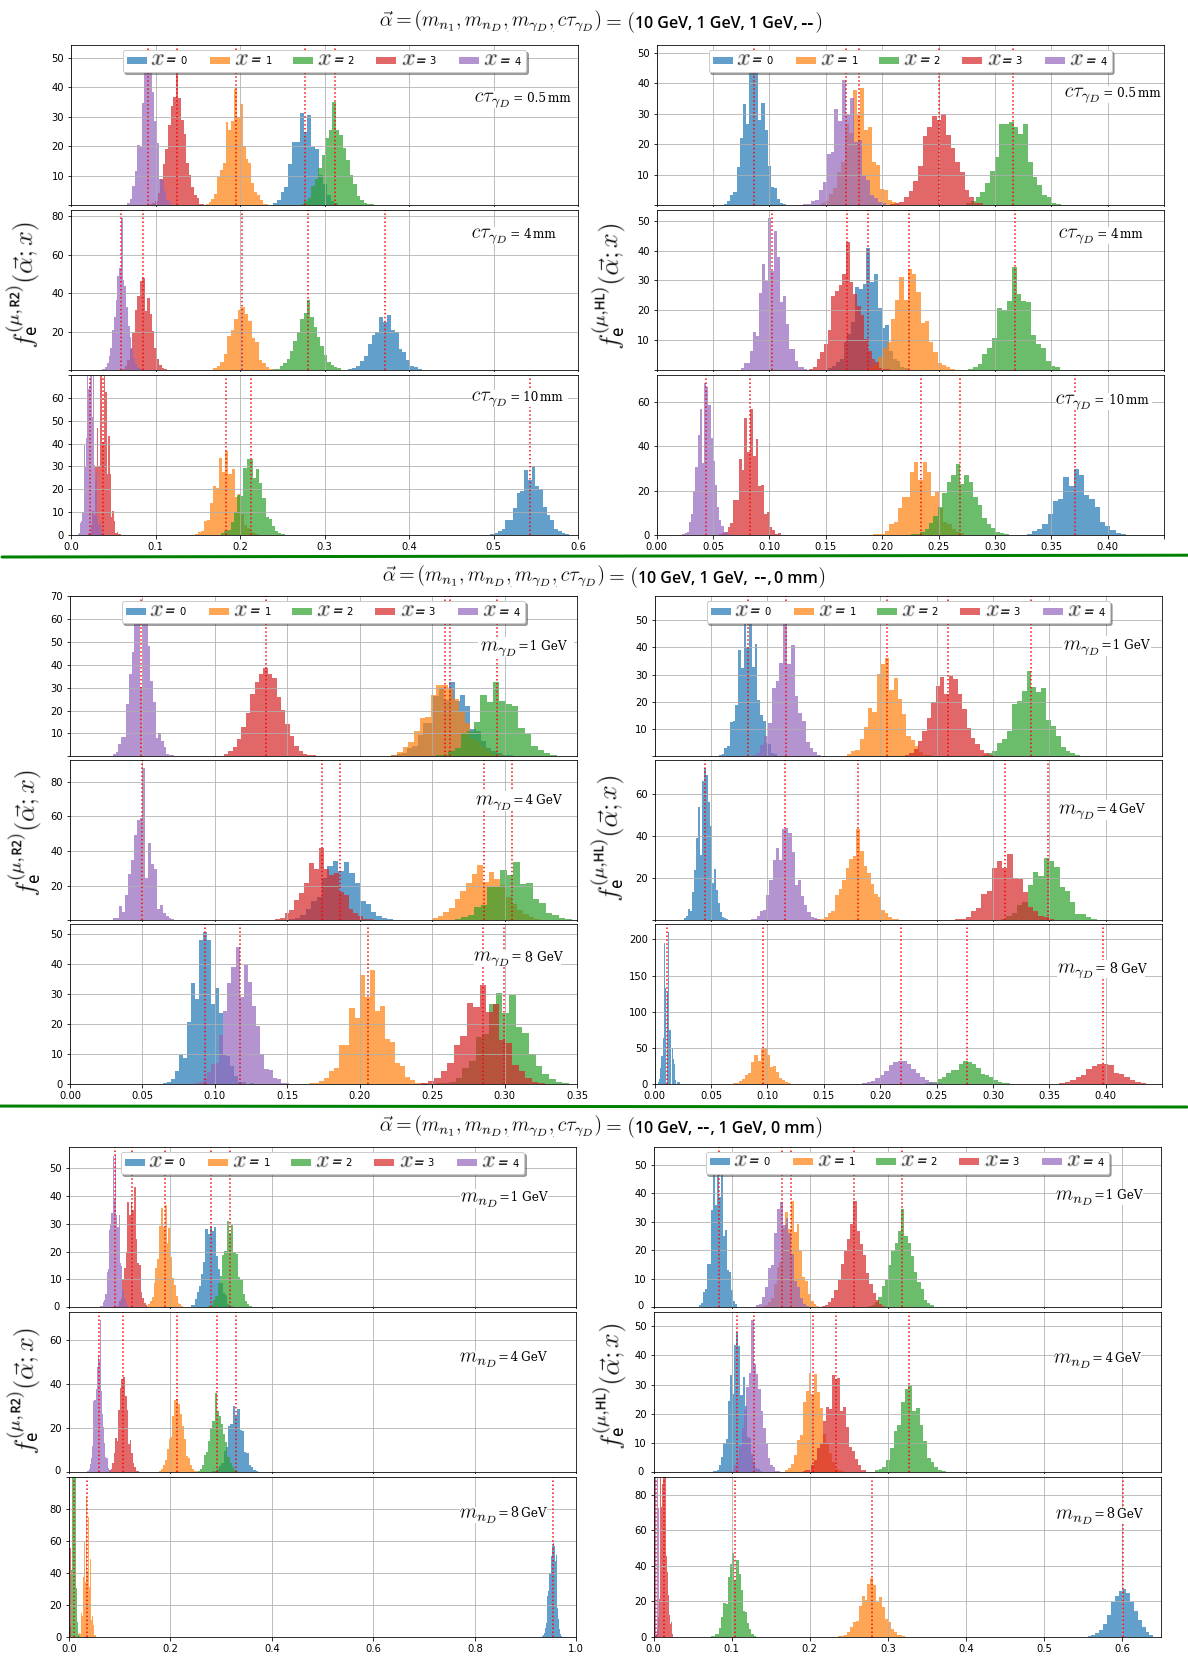
\includegraphics[width=.9\textwidth]{Simulacion/imagenes/Distribucion_Entries.png}
\caption{Distribuciones de frecuencias resultado de aplicar ``bootstrap'' sobre los valores $f^{(\mu, k)}_\textsf{e} (\vec{\alpha}; x)$ ante cambios de los parámetros $\vec{\alpha}$.}
\label{entradas}
\end{figure}

Para entender el sesgo o varianza de un estadístico genérico resultado de su aplicación sobre una población finita $\mathbb{M}$, se aplica el ``Bootstrapping''\footnote{Más información en el enlace \href{https://es.wikipedia.org/wiki/Bootstrapping\_(estad\%C3\%ADstica)}{https://\-es.\-wi\-ki\-pe\-dia.\-org/\-wi\-ki/\-Boots\-tra\-pping\_(es\-tad\-\%C3\-\%AD\-sti\-ca)}}. Este método es el resultado de la selección aleatoria de subconjuntos $\mathbb{M}_i$, seguida de la aplicación del estádistico sobre esta. La aplicación continua de ``bootstrap'' sobre el estadístico $f^{(\mu, k)}_\textsf{e} (\vec{\alpha}; x)$ y el graficar los histogramas normalizados resultantes (ver Fig. \ref{entradas}) permitirán entender la correspondencia de los términos $\vec{\alpha}$ con las distribuciones.

En las distribuciones de la Fig. \ref{entradas} muestran una alta dependencia con los parámetros $\vec{\alpha}$, además para $f^{(\mu, k)}_\textsf{e} (\vec{\alpha}; x\geqslant 5)\lesssim 0.0003$ para los cambiós de $\vec{\alpha}$ considerados en la Tabla  \ref{table_genera_v5_value}, razón por la cual son descartados de nuestra caracterización. Si consideramos que la forma de estas distribuciones corresponde con una gaussiana, el error en la frecuencia de la ec. \ref{fe} es calculable como:
%f^{(p, k)}_\textsf{e} (\vec{\alpha}; x) = \sum_{i=1}^{N_e} \delta_{x}(n_i^{(p,k)})/\sum_{i=1}^{N_e} \sum_{n=0}^\infty \delta_{n} (n_i^{(p,k)}) = \sum_{i=1}^{N_e} \delta_{x}(n_i^{(p,k)})/N_e
\begin{eqnarray}\label{error0}
\Delta f^{(\mu, k)}_\textsf{e} (x) \equiv \Delta f^{(\mu, k)}_\textsf{e} (\vec{\alpha}; x) 
& = f^{(\mu, k)}_\textsf{e} (\vec{\alpha}; x) \cdot Z_{\frac{\beta}{2}} \sqrt{\dfrac{\rho(1-\rho)}{f^{(\mu, k)}_\textsf{e} (\vec{\alpha}; x)\cdot N_e}} \\
& = \dfrac{Z_{\frac{\beta}{2}}}{100} \sqrt{\rho(1-\rho)\cdot f^{(\mu, k)}_\textsf{e} (\vec{\alpha}; x)} ~~~~~~~~~~~
\end{eqnarray}%\sqrt{\dfrac{\mathbb{E}^{(\mathtt{k})}- \mathbb{E}^{(j,~\mathtt{k})}}{\mathbb{E}^{(\mathtt{k})}-1}}
donde:\\
\begin{tabular}{lp{14cm}}
$Z_{\frac{\beta}{2}}$ & es un parámetro que depende del nivel de confianza $(1-\alpha$). Algunos de los valores mas usados son: $Z_{\frac{0.1}{2}}=1.65$, $Z_{\frac{0.05}{2}}=1.96$ y $Z_{\frac{0.01}{2}}=2.58$.\\
$\rho$ & es la probabilidad ocurrencia.
\end{tabular}

\subsubsection{Correspondencia entre los eventos de interés y los parámetros de generación.}
\begin{figure}[!t]
\centering
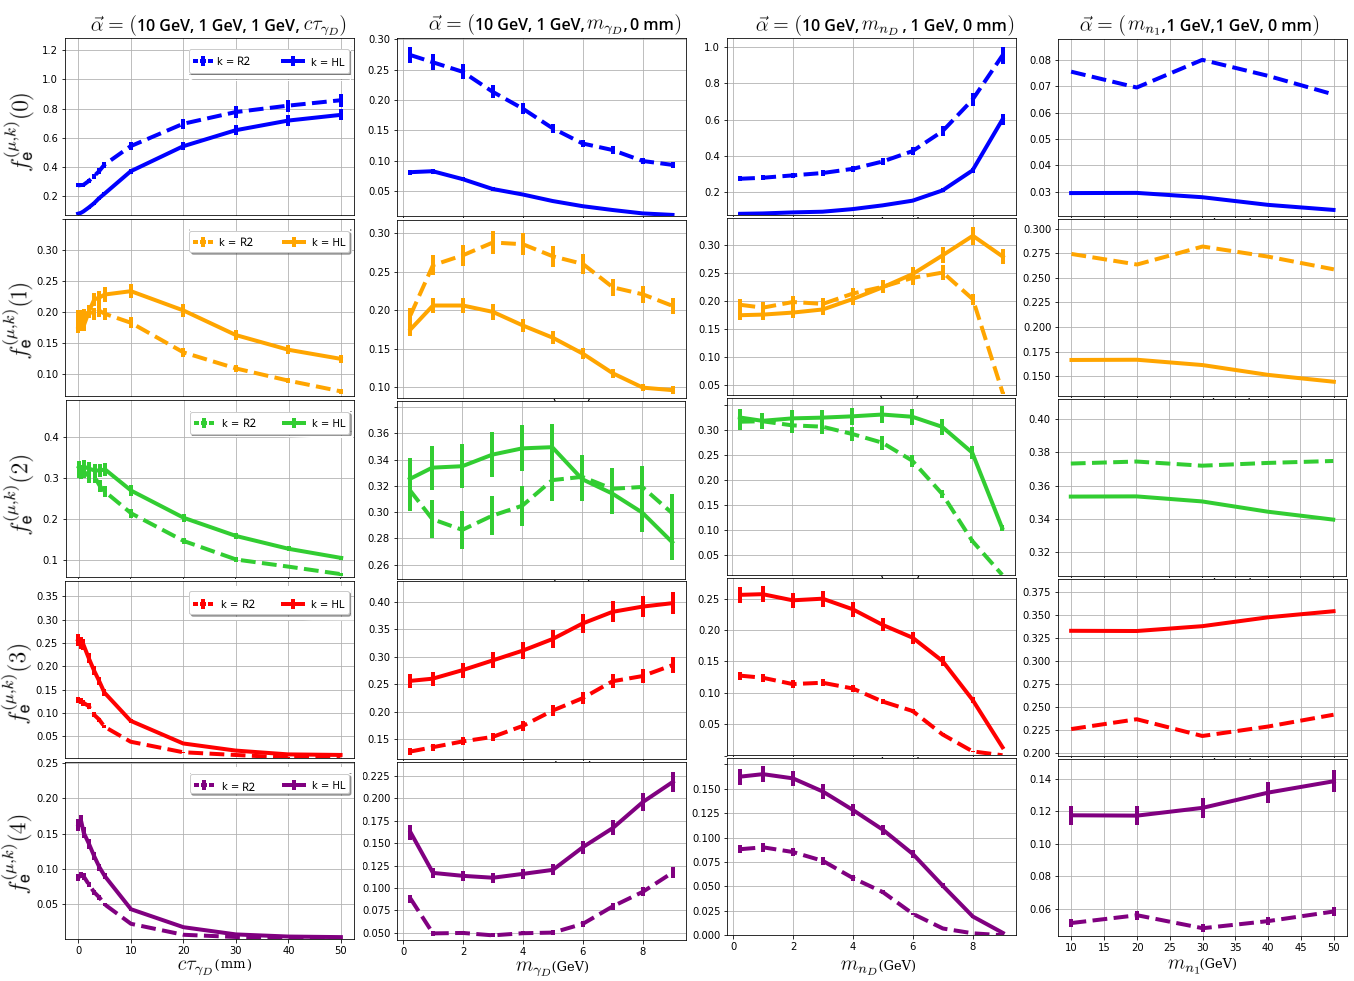
\includegraphics[width=.9\textwidth]{Simulacion/imagenes/Comparacion_Distribucion_Entries0.png}
\caption{Ejemplo de variaciones del parámetro $f^{(\mu, k)}_\textsf{e} (\vec{\alpha}; x)$.}
\label{entradasALL}
\end{figure}

Algunos ejemplos de los valores de $f^{(\mu, k)}_\textsf{e} (\vec{\alpha}; x)$ los podremos observar en la Tabla \ref{Numero_de_Entradas} y en los gráficos de la Fig. \ref{entradasALL}. En estos se puede observar una clara tendencia con los parámetros de generación $\vec{\alpha}$. Se pudo constatar la disminución de eventos de interés ($f^{(\mu, k)}_\textsf{e} (\vec{\alpha}; 4)$) con el aumento del tiempo de vida del fotón oscuro $c\tau_{\gamma_D}$ y de la masa del neutralino oscuro $m_{n_D}$, en contraste se registra aumento de los eventos de interés con la masa del fotón oscuro $m_{\gamma_D}$. En el caso de cambios de la masa del neutralino ligero $m_{n_1}$, los datos muestran variaciones pequeñas en el rango definido (ver Tabla \ref{table_genera_v5_value}), los datos adquiridos no dan una conclusión clara de su comportamiento.


% Al comparar los resultados podemos observar empíricamente una tendencia de estos valores de frecuencia ante cambios de los parámetros de generación.

%\begin{landscape}
\begin{table}[!t]
\footnotesize
\begin{tabular}{|cccccccc|}
\hline
\multicolumn{4}{|c|}{$\vec{\alpha}$} & \multicolumn{4}{|c|}{Frecuencia de muones ($f^{(\mu, \texttt{k})}_\textsf{e} (\vec{\alpha}; x) \pm \Delta f^{(\mu, \texttt{k})}_\textsf{e} (\vec{\alpha}; x)$)} \\
\hline
$m_{n_1}$ & $m_{n_D}$ & $m_{\gamma_D}$ & $c\tau_{\gamma_D}$ & 
$f^{(\mu, \texttt{R2})}_\textsf{e} (\vec{\alpha}; 0)$ & 
$f^{(\mu, \texttt{HL})}_\textsf{e} (\vec{\alpha}; 0)$ & 
$f^{(\mu, \texttt{R2})}_\textsf{e} (\vec{\alpha}; 4)$ & 
$f^{(\mu, \texttt{HL})}_\textsf{e} (\vec{\alpha}; 4)$ \\
\hline
10 & 1 & 1 & 0.5 & 0.2777 $\pm$ 0.0068 & 0.0864 $\pm$ 0.0038 & 0.0920 $\pm$ 0.0040 & 0.1678 $\pm$ 0.0053\\
& & & 2 & 0.3040 $\pm$ 0.0071 & 0.1227 $\pm$ 0.0045 & 0.0779 $\pm$ 0.0036 & 0.1355 $\pm$ 0.0047 \\
& & & 4 & 0.3718 $\pm$ 0.0078 & 0.1872 $\pm$ 0.0056 & 0.0597 $\pm$ 0.0032 & 0.1024 $\pm$ 0.0041\\
& & & 10 & 0.5428 $\pm$ 0.0095 & 0.3710 $\pm$ 0.0079 & 0.0227 $\pm$ 0.0019 & 0.0433 $\pm$ 0.0027\\
& & & 50 & 0.8570 $\pm$ 0.0119 & 0.7568 $\pm$ 0.0112 & 0.0016 $\pm$ 0.0005 & 0.0039 $\pm$ 0.0008\\
& & & 100 & 0.9217 $\pm$ 0.0123 & 0.8664 $\pm$ 0.0120 & 0.0002 $\pm$ 0.0002 & 0.0006 $\pm$ 0.0003\\
\hline
%10 & 0.25 & 0.25 & 0 & 0.2744 $\pm$ 0.0410 & 0.0813 $\pm$ 0.0223 & 0.0881 $\pm$ 0.0232 & 0.1622 $\pm$ 0.0315 \\
10 & 1 & 2 & 0 & 0.2467 $\pm$ 0.0064 & 0.0699 $\pm$ 0.0034 & 0.0497 $\pm$ 0.0029 & 0.1135 $\pm$ 0.0043 \\
& & 4 & & 0.1862 $\pm$ 0.0055 & 0.0446 $\pm$ 0.0027 & 0.0494 $\pm$ 0.0029 & 0.1157 $\pm$ 0.0040 \\
& & 6 & & 0.1286 $\pm$ 0.0046 & 0.0253 $\pm$ 0.0021 & 0.0599 $\pm$ 0.0032 & 0.1456 $\pm$ 0.0049\\
& & 8 & & 0.0998 $\pm$ 0.0040 & 0.0134 $\pm$ 0.0015 & 0.0957 $\pm$ 0.0040 & 0.1960 $\pm$ 0.0057\\
\hline
10 & 2 & 1 & 0 & 0.2929 $\pm$ 0.0069 & 0.0890 $\pm$ 0.0038 & 0.0852 $\pm$ 0.0038 & 0.1604 $\pm$ 0.0052\\
& 4 & & & 0.3287 $\pm$ 0.0074 & 0.1072 $\pm$ 0.0042 & 0.0586 $\pm$ 0.0031 & 0.1281 $\pm$ 0.0046 \\
& 6 & & & 0.4265 $\pm$ 0.0084 & 0.1536 $\pm$ 0.0051 & 0.0221 $\pm$ 0.0019 & 0.0831 $\pm$ 0.0037\\
& 8 & & & 0.7097 $\pm$ 0.0108 & 0.3203 $\pm$ 0.0073 & 0.0022 $\pm$ 0.0006 & 0.0193 $\pm$ 0.0018\\
\hline
20 & 1 & 1 & 0 & -- & -- & 0.0560 $\pm$ 0.0030 & 0.1176 $\pm$ 0.0044 \\
30 & & & &  --  & -- & 0.0480 $\pm$ 0.0028 & 0.1224 $\pm$ 0.0045\\
40 & & & & -- & -- &  0.0524 $\pm$ 0.0030 &  0.1319 $\pm$ 0.0047 \\
50 & & & & -- & -- & 0.0583 $\pm$ 0.0031 & 0.1391 $\pm$ 0.0048 \\
\hline
\end{tabular}
\caption{Valores de $f^{(\mu, \texttt{k})}_\textsf{e} (\vec{\alpha}; x)$ para combinaciones de los términos del parámetro generación $\vec{\alpha}$ y los detectores $k$.}
\label{Numero_de_Entradas}
\end{table}

Dado que se intenta reconstruir el decaimiento de la Fig. \ref{fig:sketch_darksector}b, el estadístico $f^{(\mu, \texttt{HL})}_\textsf{e} (\vec{\alpha}; 4)$ es el de mayor interés para esta investigación, el mismo muestra como la configuración del detector en Alta Luminosidad ($k=\textsf{HL}$) reconstruye entre 86.7\%-790.2\% más de eventos con 4 muones que el detector en la configuración Run-2 ($k=\textsf{R2}$) para las muestras simuladas (ver Tabla \ref{table_genera_v5_value}).





\subsubsection{Regresión de datos de frecuencia $f^{(\mu, k)}_\textsf{e} (\vec{\alpha}; x)$.}

Con la intención de realizar una caracterización eficiente de la cantidad de eventos de interés y de su dependencia con los parámetros de generación, se intenta utilizar métodos simples de regresión para valorar la posibilidad de inferir información pertinente a la frecuencia de los eventos. Para esto se utilizán los métodos presentados ya en la seccion \ref{Cap_regresion} mediante una aproximación lineal como la propuesta en la ec. \ref{regresion} y con una red neuronal como la presentada en la Fig. \ref{neuronas}.

\begin{figure}[!ht]
\centering
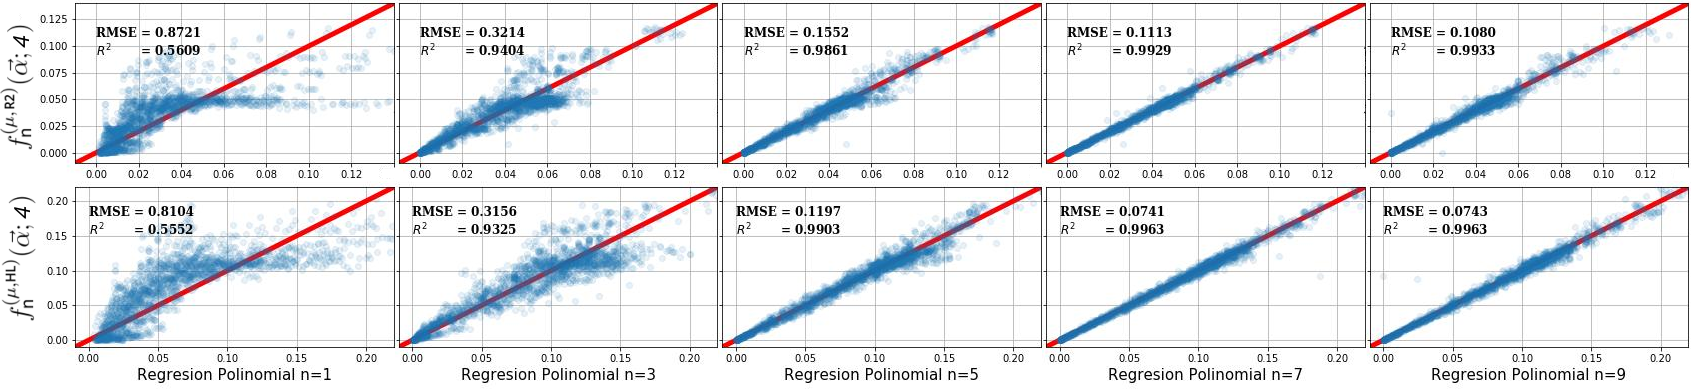
\includegraphics[width=1\textwidth]{Simulacion/imagenes/ML_Entries3.png}
\caption{Resultados de la regresión polinomial de los valores de frecuencia $f^{(\mu, k)}_\textsf{e} (\vec{\alpha}; 4)$.}
\label{regresionALL}
\end{figure}


Al implementar el método de regresión polinomial sobre los datos 
$f^{(\mu, k)}_\textsf{e} (4)$ 
hasta el orden $n = 9$ en la Fig. \ref{regresionALL}, se puede observar una mejora en los parámetros progresiva con el aumento del orden $n$. Se visualiza con facilidad la correspondencia entre los valores simulados y los predichos, esta es corrobarada por los parámetros de confianza \textbf{RMSE} y $\mathbf{R^2}$. 

Haciendo uso del método \textbf{RNA} según una configuración semejante a la Fig. \ref{regresion} con $4$ capas ocultas con cantidad de nodos $m_k=\{9,~7,~5,~3\}$ por cada uno respectivamente, se obtuvo un modelo con valores de \textbf{RMSE} y $\mathbf{R^2}$ comparables con los del método de regresión lineal explicado con anterioridad.

\begin{figure}[!ht]
\centering
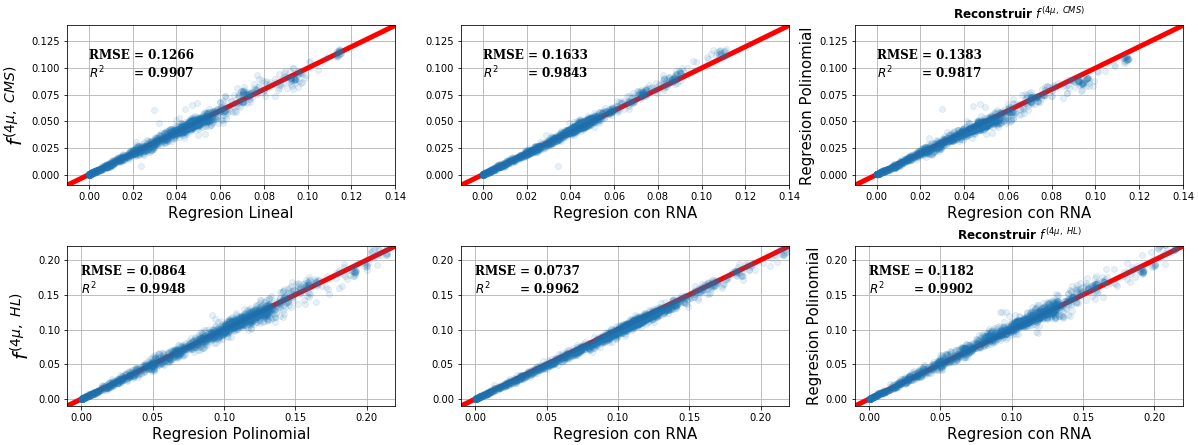
\includegraphics[width=1\textwidth]{Simulacion/imagenes/ML_Entries.png}
\caption{Comparación de los resultados de regresión utilizando RNA y regresión polinomial para predecir las frecuencias $f^{(\mu, k)}_\textsf{e} (\vec{\alpha}; 4)$.}
\label{regresionALL1}
\end{figure}

En la Fig. \ref{regresionALL1} también se puede observar una comparación de los resultados de los dos métodos al intentar reconstruir la información de los valores de frecuencia $f^{(4\mu,~k)}$ mostrando una alta linealidad en los resultados obtenidos válidando su implementación como método de análisis. Los resultados dan claridad de como el método de predicción del porciento de eventos con 4 muones puede ser utilizado para optimizar la selección del parámetro $N_e$ en el proceso de generación (ver Tabla \ref{table_genera_v5_value}).

%Al analizar los errores de estás predicciones con los datos originales se obtuvo que lo resultados diferencian hasta en un $\sim 30\%$, siendo una de las posibles consecuencias de estos altos errores el pequeño valor del parámetro de generación \texttt{Event} (ver sección \ref{Cap_genera}).

%\begin{landscape}
%\begin{figure}[h]
%\centering
%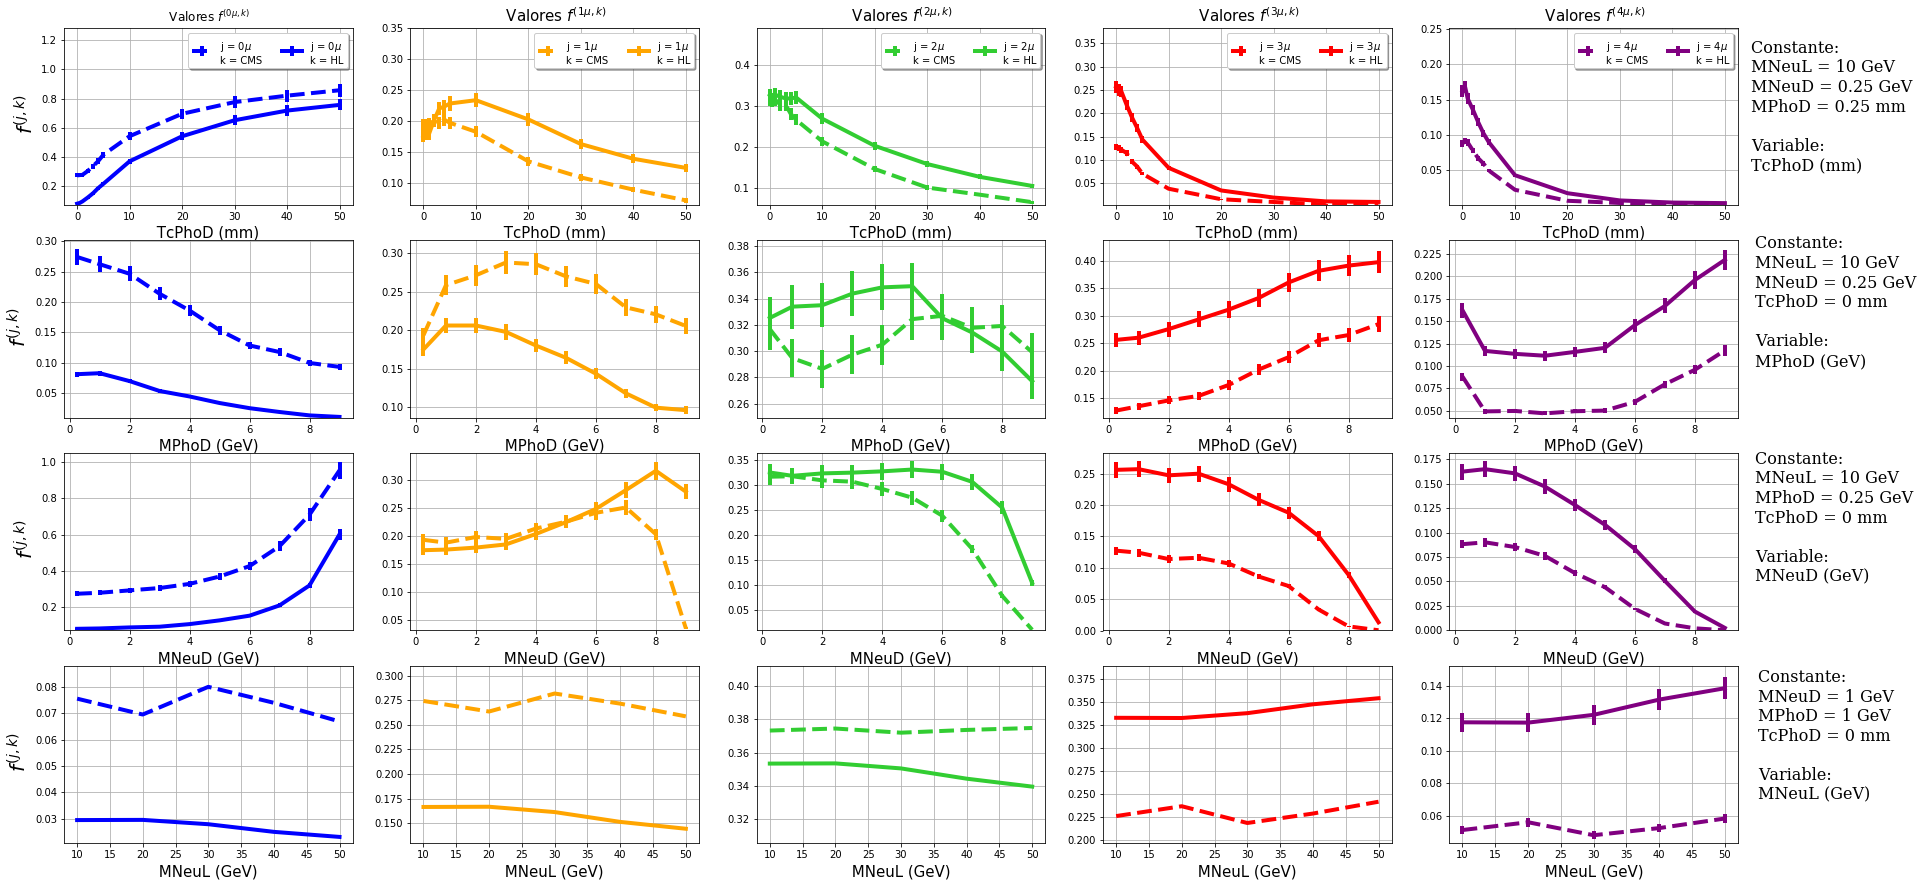
\includegraphics[width=1.2\textwidth]{Simulacion/imagenes/Comparacion_Distribucion_Entries.png}
%\caption{Distribuciones de frecuencia de las entradas $f^{(j,~k)}$ ante cambios de \texttt{MNeuD}.}
%\label{entradasALL}
%
%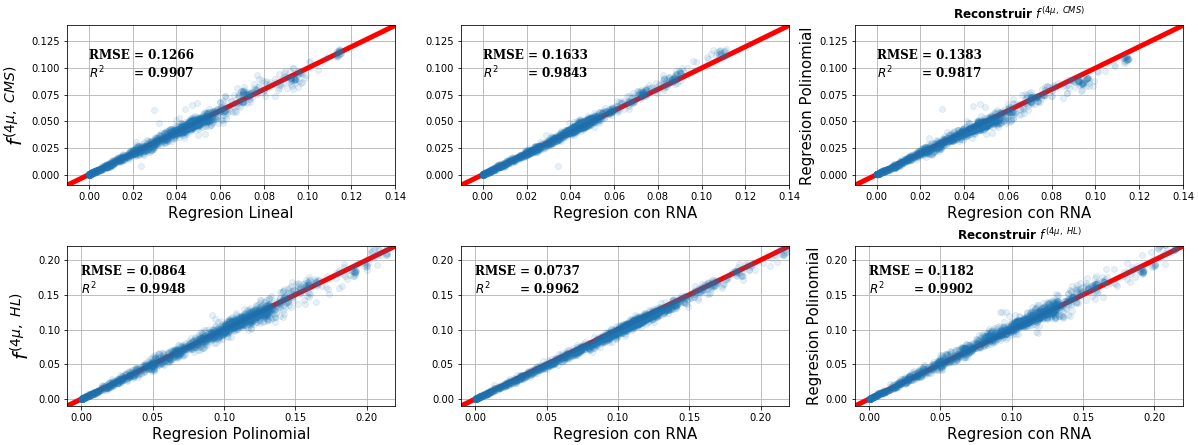
\includegraphics[width=1\textwidth]{Simulacion/imagenes/ML_Entries.png}
%\caption{Resultados de la regresión de los valores de frecuencia $f^{(4\mu,~k)}$.}
%\label{regresionALL}
%\end{figure}
%\end{landscape} 


%\subsubsection{Probabilidad de ocurrencia.}

%Para cierta combinación de parámetros, los detectores en sus diferentes configuraciones tienen una probabilidad $p$ de ocurrencia o reconstrucción del muón, si se hace la suposición de que esta probabilidad es fija para cierta morfologia en las propiedades de los muones entonces podemos hacer uso de la binomial para facilitar las comparaciones entre los eventos.
%Partiendo de la ecuación binomial:
%\begin{equation}\label{binomial}
%f^{(j,~k)} = \dfrac{n_{max}!}{n_j!~(n_{max} - n_j)!} ~ p^{n_j} ~ (1-p)^{n_{max}-n_j}
%\end{equation}
%donde:\\
%\begin{tabular}{lp{14cm}}
%$n_{j} = j$ & número de muones. Para nuestras muestras los valores admisibles son $j = \{0,~1,~2,~3,~4\}$, resultado de lo cual $n_{max} = n_{4\mu} = 4$. \\
%$p$ & es la probabilidad ocurrencia o reconstrucción de los muones.
%\end{tabular}
%Dado que el $\backsim 80\%$ de los datos generados a los que se tiene acceso solo se posee información de los eventos $\mathbb{E}^{(4\mu,~\mathtt{k})}$, entonces podemos calcular la probabilidad de ocurrencia como:
%\begin{equation}\label{ocurrencia}
%f^{(4\mu,~k)} = \dfrac{4!}{4!~0!} ~ p^{4} ~ (1-p)^{0} = p^{4} ~~~\Rightarrow ~~~ p = \sqrt[4]{f^{(4\mu,~k)}}
%\end{equation}
%
%Finalmente sustituyendo la ec. \ref{ocurrencia} en ec. \ref{binomial} tenemos:
%\begin{equation}\label{binomialF}
%f^{(j,~k)} = \dfrac{n_{max}!}{n_j!~(n_{max} - n_j)!} ~ (f^{(4\mu,~k)})^{\frac{n_j}{4}} ~ (1-(f^{(4\mu,~k)})^{\frac{1}{4}})^{n_{max}-n_j}
%\end{equation}
%Con esta ecuación se podrá simular los valores $f^{(j,~k)}$ para los datos con información reducida, aunque dada las suposiciones que deriban de esta ecuación los errores observados de la comparación con los datos reales pueden llegar a $20\%
%,$.%$\Delta f^{(j,~k)} / f^{(j,~k)} = 20\%$ 
%
%
%
%
%


\subsection{Variación de las propiedades de los muones con el parámetro $\alpha$*}
La caracterización de las propiedades de los muones es parte importante de este estudio, obtener las dependencias empíricas entre ellas y los posibles cambios en los límites de estas propiedades resultado del cambio de la eficiencia de los detectores en sus diferentes configuraciones se hace necesario para comprender mejor como se visualiza la teoría investigada desde su reconstrucción por los detectores.



Ante la necesidad de hacer estadística con las variables $\chi$ definimos la frecuencia de cada una de estas variables $\mathbb{F}_\chi^{(\mathtt{k})}$(x) donde para un valor predefinido de resolución de la información $\delta \chi$
\begin{equation}
\mathtt{\Theta(X,~Y)} ~ = ~ \Bigg\{\begin{matrix}
1 & \mathtt{X-\Delta X ~<~Y ~and~Y~ < X+\Delta X}\\
0 & \mathtt{X-\Delta X ~>~Y ~~or~~Y~ > X+\Delta X}
\end{matrix} 
\end{equation}

\begin{equation}
\mathbb{F}_\chi^{(\mathtt{k})} (x)= \sum_{ji} \mathtt{\Theta}(\chi_i^{(j,k)},~x)
\end{equation}

\begin{equation}
f_\chi^{(\mathtt{k})} (x)= \mathbb{F}_\chi^{(\mathtt{k})} (x)/ \sum_x \mathbb{F}_\chi^{(\mathtt{k})} (x)
\end{equation}


%\texttt{MNeuL}, \texttt{MNeuD}, \texttt{MPhoD}, \texttt{TcPhoD})




En los gráficos superiores de la Fig. \ref{procesos_darksusy_PTyISO} se puede observar los valores de momento angular de todos los muones reconstruidos para eventos $\mathbb{E}_i^{(4\mu,~\mathtt{CMS})}$ (configuración \texttt{Run-2}) y $\mathbb{E}_i^{(4\mu,~\mathtt{HL})}$ (configuración en \texttt{High Luminosity}), en estos se puede visualizar las diferencias entre los rangos de detección donde para eventos $k=$\texttt{CMS} el $\backsim ~ 99\%$ de los muones poseen $\sim 10  < ~ P_t^{(4\mu,~\mathtt{CMS})} ~ <\sim 100$, en contraste para $k=$\texttt{HL} tenemos $\sim 0.1 < ~ P_t^{(4\mu,~\mathtt{HL})} ~ < \sim 100$. Este aumento de rango en \texttt{HL} para valores menores de $\backsim ~ 10~GeV$ se puede ver que no es sin pérdidas, se puede constatar un cambio en la forma de los gráficos, esto es debido a que la inclusión de nuevos sensores en la configuración \texttt{HL} no poseen la misma eficiencia en la reconstrucción de la información.

\begin{figure}[!ht]
\centering
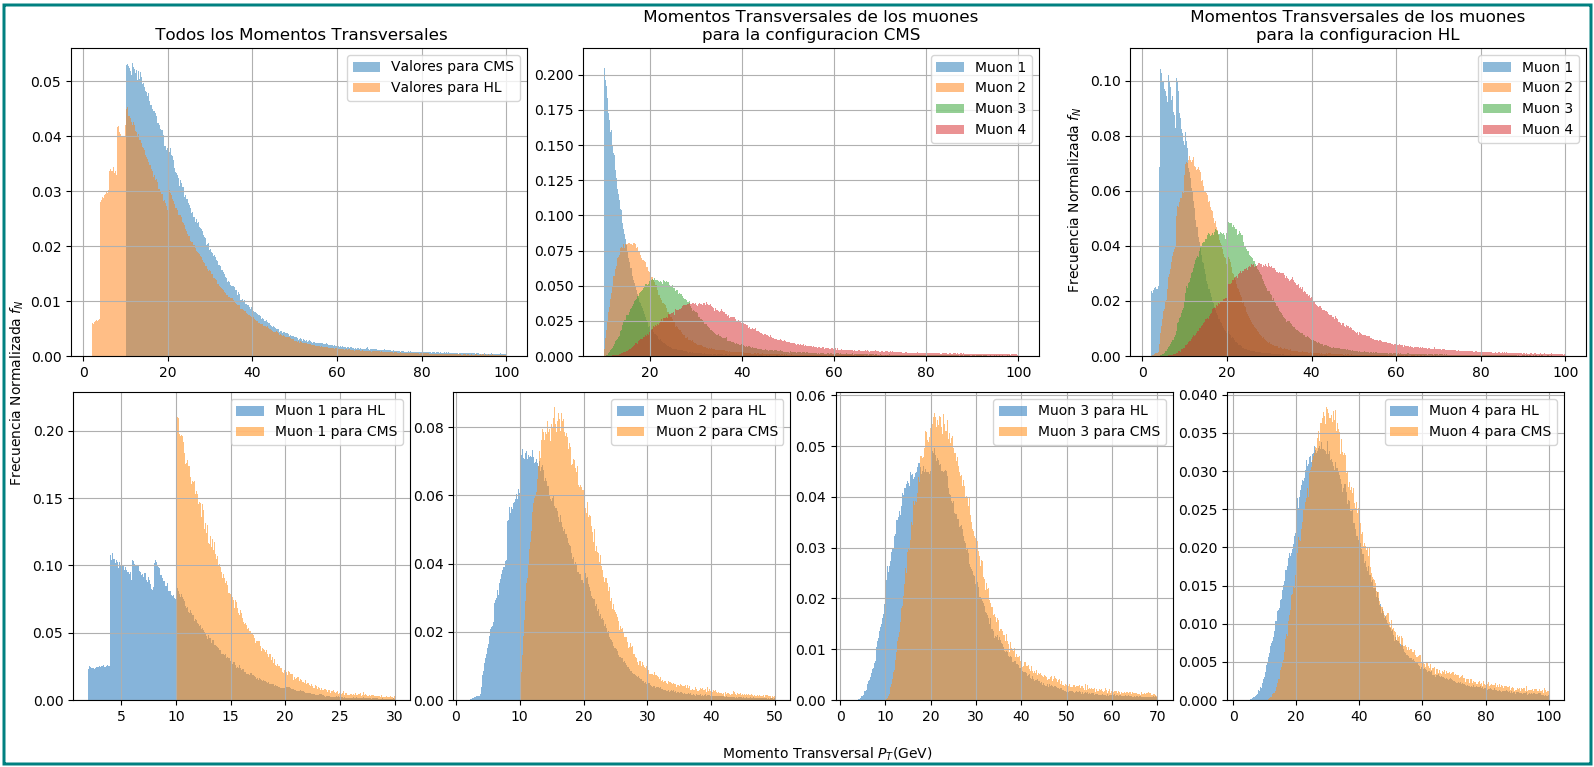
\includegraphics[width=.8\textwidth]{Simulacion/imagenes/Datos_PT_ALL.png}
%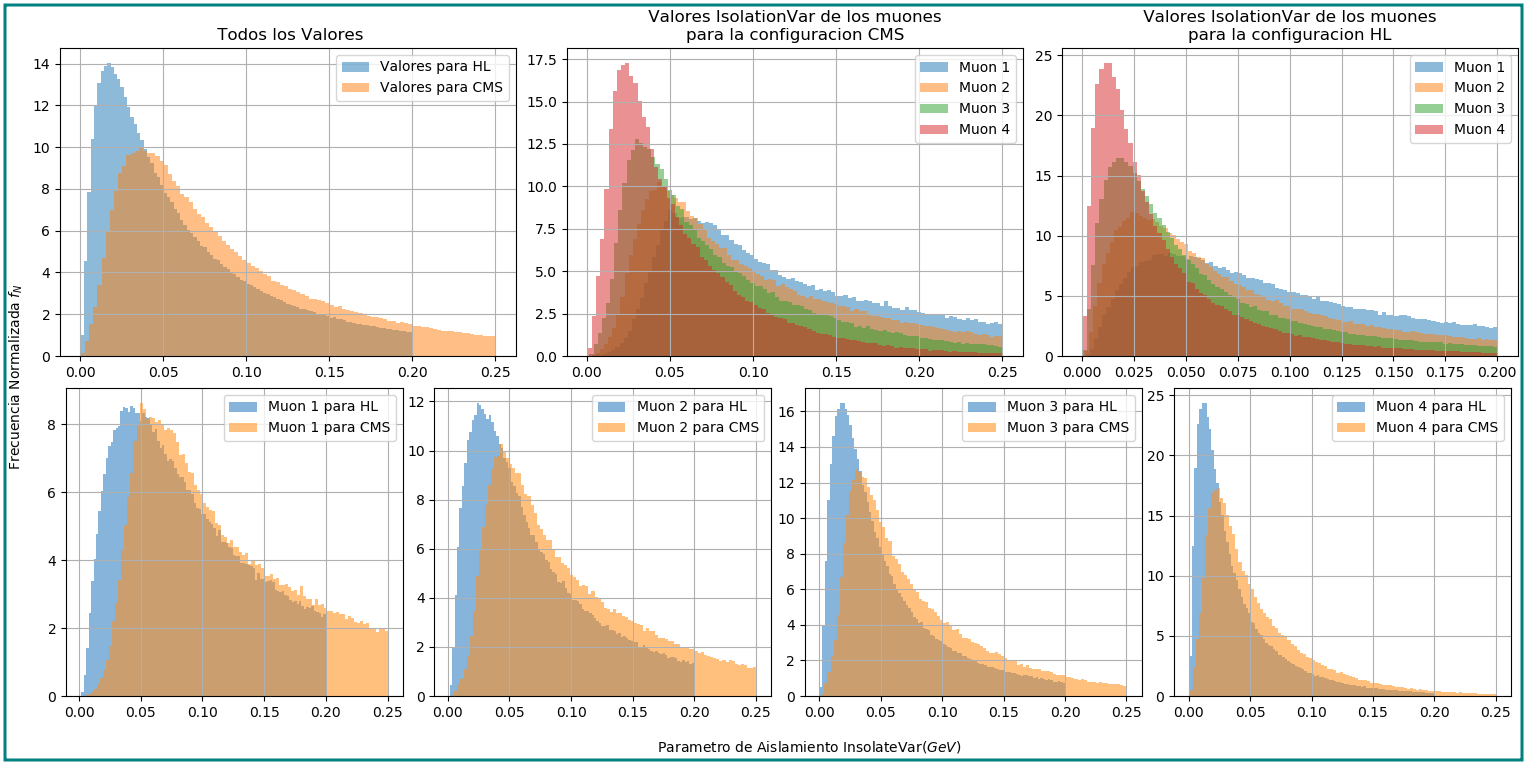
\includegraphics[width=.8\textwidth]{Simulacion/imagenes/Datos_IsolationVar_ALL.png}
\caption{Caracterización global de los momentos transversales de nuestra población de muones reconstruidos.}
\label{procesos_darksusy_PTyISO}
\end{figure}



\subsubsection{Valores de angulo}
\begin{figure}[!ht]
\centering
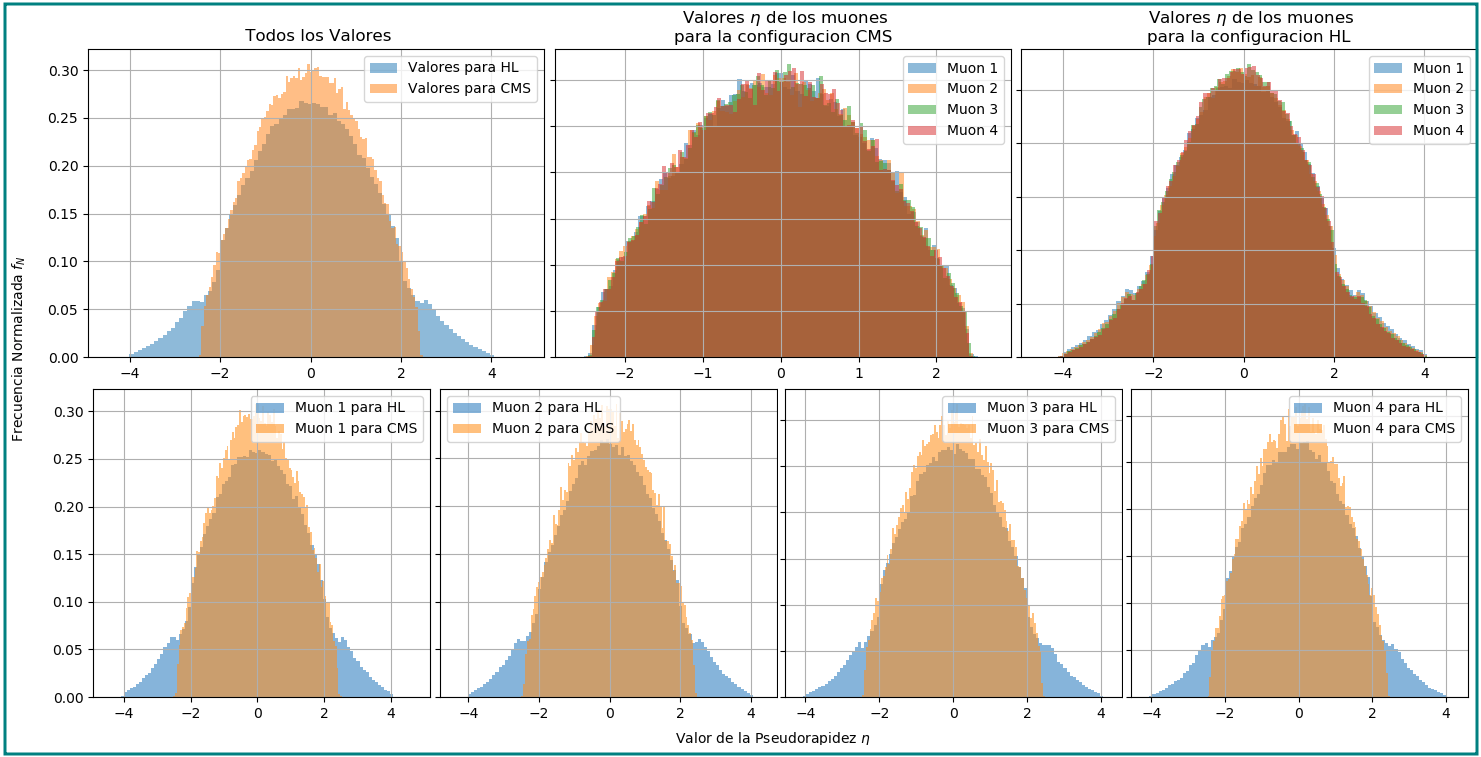
\includegraphics[width=.8\textwidth]{Simulacion/imagenes/Datos_Eta_ALL.png}
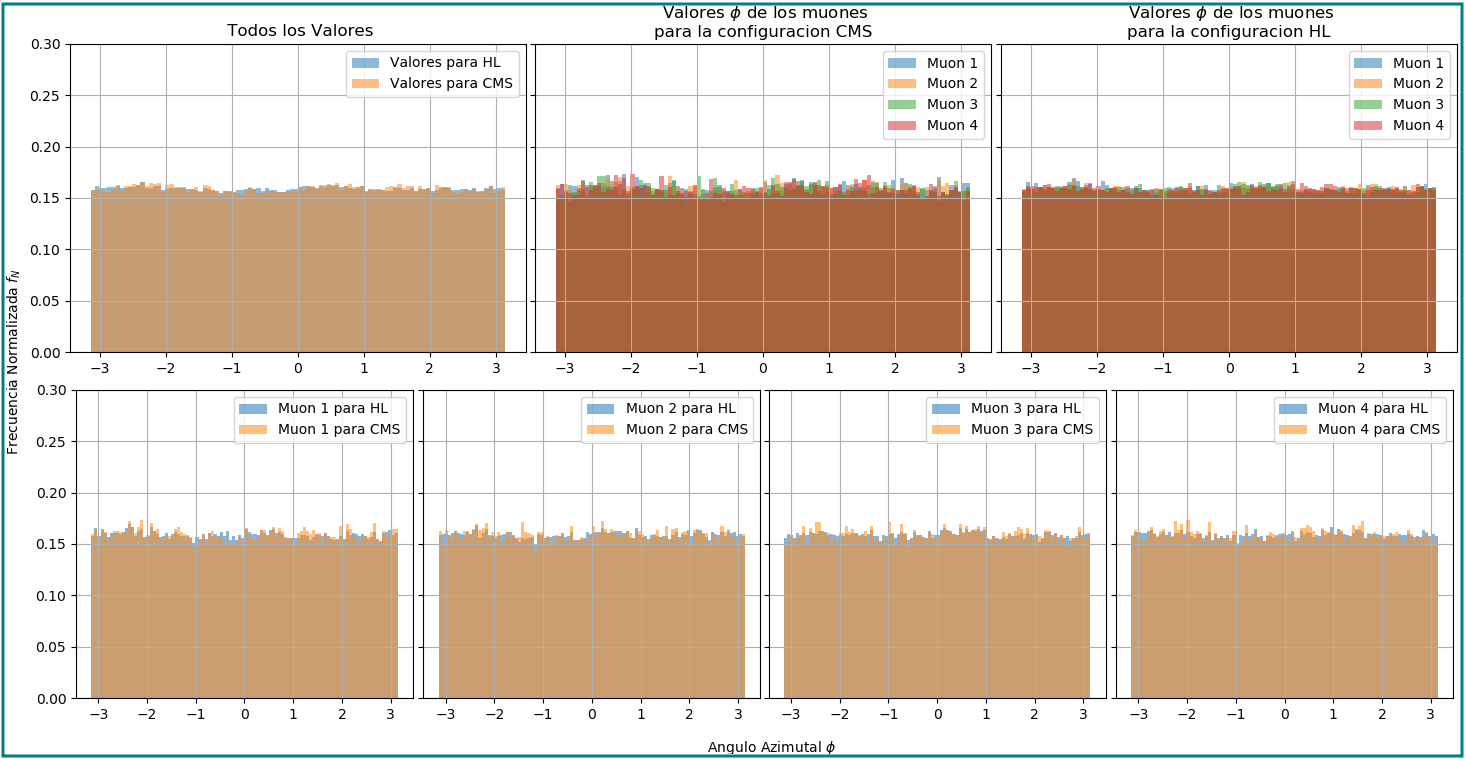
\includegraphics[width=.8\textwidth]{Simulacion/imagenes/Datos_Phi_ALL.png}
\caption{Grupo total de datos generados para los eventos de interes.}
\label{procesos_darksusy_ETAyPHI}
\end{figure}





Otro factor importante en la detección de los muones es el valor de Entonces de forma generar se puede Además como límite superior se puede constatar que el  se encuentran para valores 


\subsection{Reconstruyendo el fotón oscuro $\gamma$*}











